\section{SSP Basis Sets}
\label{891_2:sec:SSP_sets}

Generating synthetic spectra that fit our data in a $\chi^2$ sense is
not very difficult or illuminating. A ``good'' fit is good only in the
sense that a collection of SSPs was added together with a set of
weights (Equation \ref{891_2:eq:SSP_galaxy}) that reproduce the spectrum of
our galaxy with a reasonable degree of accuracy. Degeneracies between
SSPs that have different underlying ages or metallicities but similar
spectra (and therefore can contribute equally to ``good'' fits) make
an accurate recovery of SFH, age, and metallicity difficult. To
maximize the amount of information we get from full-spectrum fits we
need to use an SSP library that a) produces ``good'' fits, and b)
minimizes internal degeneracies to increase the precision on derived
parameters (i.e., SFH, age, metallicity, and extinction).

In this section explore different methods of combining information
from SSPs with different ages and metallicities
(\S\ref{891_2:sec:bc03_SSP}). We then discuss a statistically motivated way
to reduce the number of free parameters in our figs
(\S\ref{891_2:sec:bc03_dfk}) and examine systematic differences between
different SSP libraries (\S\ref{891_2:sec:ma11}). The final SSP library used
for analysis of NGC 891 is discussed in \S\ref{891_2:sec:final_SSP}.

Before any analysis, all model SSPs are degraded to match the spectral
resolution of our data. As discussed in \ref{chap:891_1} this
resolution is a function of both \GP fiber size and wavelength.

%++++++++++++++++++==
%% {\bf MAB: I would say this differently. First I would expound on that
%%   nature of SPS as a weighted sum of SSPs that reflect an assumed,
%%   constrained, or otherwise simulated SFH and extinction (refer back
%%   to your eqn. 1). Being able to produce a good SPS fit to the
%%   observed spectra is a necessary but not sufficient condition to
%%   achieve astrophysical insight in to the SFH, and hence and and
%%   metallicity distributions, because of the inherent degeneracies in
%%   the SPS fitting, specifically in the trade-offs between different
%%   SSP weights that have sigificant impact on inferred astrophysical
%%   properties (SFH and Z), but yield the same quality spectral fit. As
%%   a consequence, the first order of business is to determine if the
%%   necessary condition can be met (and if different SPS are a major
%%   issue for our observed data and wave range), and then to figure out
%%   how to minimize the degeneracy in a way that exploits real
%%   information in the spectra. What the latter means is not fooling
%%   ourselves about resolving SFH over age ranges where we have no
%%   diagnostic power, namely, at older ages.

%%   Then you want to give a road-map to the remainder of the
%%   section. You give a bit in 5.1, but let's put it all up
%%   front. Something like...

%%   In this section we explore the impact of fitting mono-Z vs multi-z
%%   (word this better) with the aim or criteria of X and Y. Attempts to
%%   make a more sophisticated stellar pop. age-dependent extinction
%%   model.  The above are a motivation for a down select based on
%%   something known as DFK. We also checked other SPS models to explore
%%   systematics, and then conclude on our final choice.

%% }

\subsection{Variations in Treating Metallicity and
  Extinction}
\label{891_2:sec:bc03_SSP}
The first class of SSPs used all come from \citet{Bruzual03}
(hereafter \citetalias{Bruzual03}) and use the the same 10 age bins
used by \citet{Tremonti04} (in Gyr: 0.005, 0.025, 0.1, 0.286, 0.64,
0.904, 1.434.2.5, 5, and 10).  Within these ages we also explored six
metallicities (\val{0.005}{\Zsol}, \val{0.02}{\Zsol},
\val{0.2}{\Zsol}, \val{0.4}{\Zsol}, \val{1}{\Zsol}, and
\val{2.5}{\Zsol}).

Using this basis set we tried three different mixing/fitting methods,
described below.

\subsubsection{Mono-Metallicity SSPs}
\label{891_2:sec:mono_metal}

The most basic libraries we used are 10 SSPs corresponding to the ages
listed above all at a single metallicity. To probe different
metallicities we constructed a single library for each of the six
metallicities listed above and ran separate fits for each one. The
final ``best'' metallicity value in each aperture was then determined
to be the mono-metallicty fit with the lowest $\chi^2_\nu$ value.
Assuming that all the separate metallicity fits represent the same
underlying photon distribution (i.e., NGC 891) and therefore sample
from the same $\chi^2$ distribution (one that contains the ``correct''
model) we can compute a confidence limit in metallicity space by
considering $\Delta\chi^2$. Here $\Delta\chi^2$ is simply the
difference in $\chi^2$ for each metallicity from the metallicity with
the lowest $\chi^2$ value. Following the example of \citet{Wall03},
the probability that a best fit with value $\chi^2 = \chi^2_i$ comes
from the same distribution (and is therefore a valid fit) as a model
with $\chi^2 = \chi^2_{\mathrm{min}}$ is\footnote{$\Delta\chi^2$ and
  Equation \ref{891_2:eq:chi_cdf} do \emph{not} correspond to reduced
  $\chi^2$. In practice all of our fits have the same number of
  degrees of freedom so this distinction is irrelevant.}
\begin{equation}
\label{891_2:eq:chi_cdf}
\alpha(\Delta\chi^2,k) = \int_0^{\Delta\chi^2}\frac{t^{(k-2)/2}e^{-t/2}}{2^{k/2}\Gamma (k/2)}dt
\end{equation}
where $\Delta\chi^2 = \chi^2_i - \chi^2_{\mathrm{min}}$, $k$ is the number of
free parameters, and $\Gamma$ is the gamma function. Equation \ref{891_2:eq:chi_cdf}
is simply the cumulative distribution function of the $\chi^2$ distribution.

Once the probabilities have been computed we reject any metallicities
with $\alpha < 0.68$. The final reported age is then the average of
$\tau_L$ over the remaining metallicities and a good estimate of the
uncertainty in $\tau_L$ caused by degeneracy in metallicity is the
corresponding standard deviation. 

%% {\bf MAB: The above is very nicely described. Do we want to say
%%   anything here about whether we think the approach yields reasonable
%%   results, i.e., is a plausible statistical models? I am thinking
%%   about this sentence: ``...all the separate metallicity fits come
%%   from the same $\chi^2$ distribution (one that contains the
%%   ``correct'' model)...''  What is the ``fit''? Is it the model
%%   constructed out of N weights for the different SSP ages of a given Z
%%   plus an attenuation? Is there anything about the fits that we accept
%%   or reject that might lead us to believe the statistical criterion is
%%   reasonable?}

One drawback of this fitting method is that SSPs of all ages are
forced to have the same metallicity. Additionally, while different
apertures are allowed to have different metallicities, the metallicity
resolution is constrained to the grid of metallicities defined in
\citet{Bruzual03}.

\subsubsection{Multi-Metallicity SSPs}
\label{891_2:sec:multi_metal}
To address the metallicity issues mentioned above we next explored an
SSP library that sampled all SSP ages and metallicities
\emph{simultaneously}. In other words, each age bin of stars was
allowed to contribute flux from an arbitrary combination of SSPs at
different metallicities; instead of fitting 10 ages six times (one for
each metallicity) we now fit 60 SSPs (10 ages times 6 metallicities)
all at once. The reported metallicity is the the mean, light-weighted
metallicity described in Equation \ref{891_2:eq:MLWZ}.

\begin{figure}
  \centering
  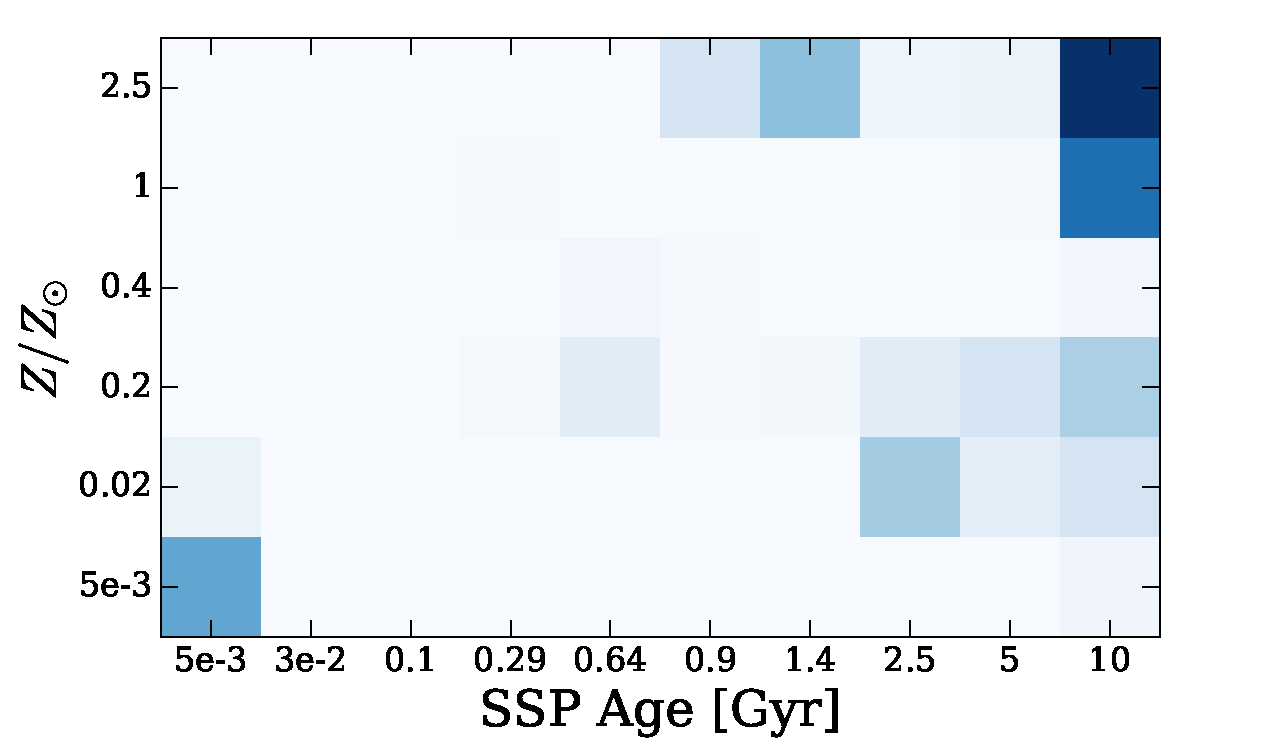
\includegraphics[width=\columnwidth]{891_2/figs/allZ2_all_weights.pdf}
  \caption[Example of SSP ligh-weights for 61 parameter
    fit]{\fixspacing\label{891_2:fig:multiZ_weights}SSP light weights
    across all apertures in all pointings for the multi-metallicity
    SSP basis set. Each square shows the light weight, $W_{L,i,j}$,
    for SSP age $t_i$ and metallicity $Z_j$, averaged across all 261
    apertures. Before averaging each aperture is normalized to the
    same total flux so that the darkness of the box represents a true
    comparison of the relative contributions of each SSP across the
    all apertures.}
\end{figure}

Unlike the mono-metallicity libraries our multi-metallicity SSP
library allows fore a more physically realistic picture NGC 891, one
in which each location in the galaxy is a superposition stellar
populations with different formation ages and metallicities. This
additional information comes at a cost, however; 60 free parameters
(plus one for the extinction) can leady to degeneracies that severely
dilute our ability to precisely interpret the results of our fits.

\begin{figure}
  \centering
  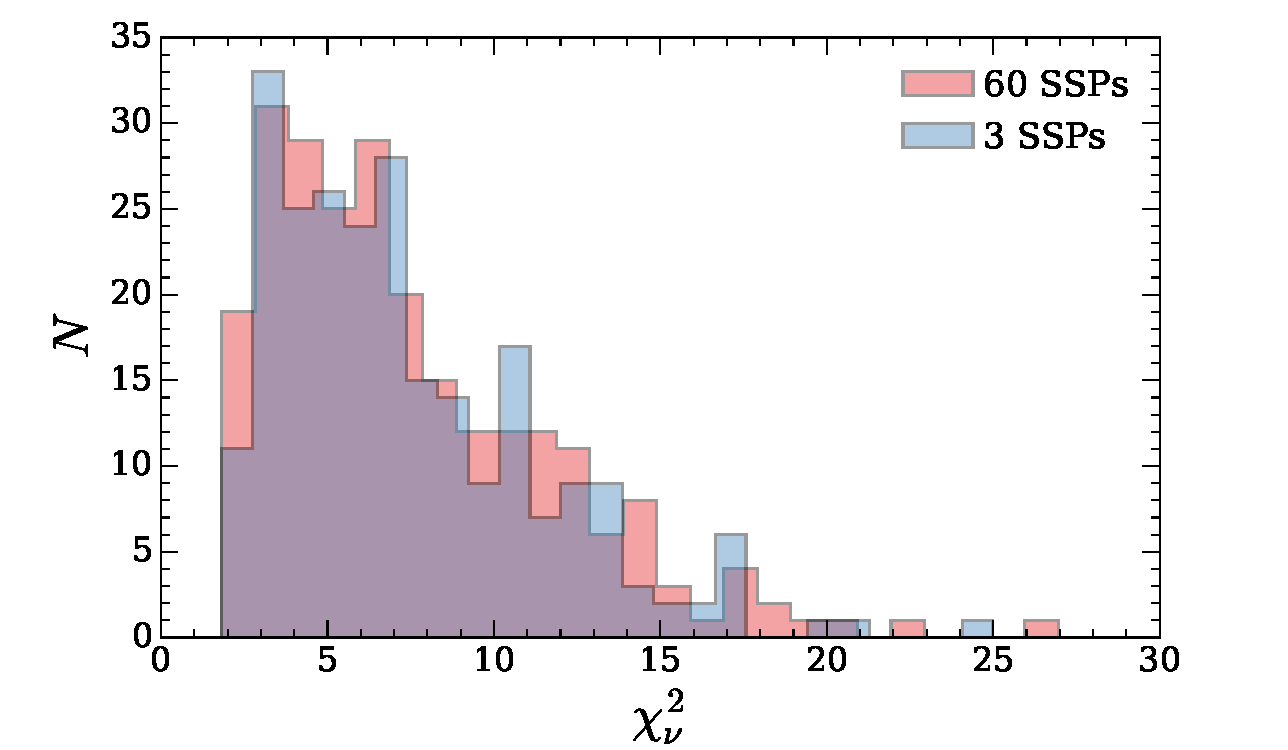
\includegraphics[width=\columnwidth]{891_2/figs/allz_chihist.pdf}
  \caption[$\chi_{\nu}^2$ distribution for 61 and 4 parameter
    fits]{\fixspacing\label{891_2:fig:3SSP_chi}Distribution of
    best-fit $\chi^2_\nu$ values for the full, multi-metallicity basis
    set described in \S\ref{891_2:sec:multi_metal} (\emph{red}) and a
    artificially down-selected basis set containing only 5, 904, and
    \val{1000}{Myr} SSPs 1 \Zsol (\emph{blue}). A 2-sample KS test
    indicates these two distributions come from the same underlying
    distribution with $p > 0.99$.}
\end{figure}

Figure \ref{891_2:fig:multiZ_weights} shows an example of the
age/metallicity parameter space spanned by this method. We find that
60 SSPs generally overconstrain the spectral fitting and only \asim 5
SSPs contribute significant flux. To further investigate these
degeneracies we constructed a test basis set that contained only 3 of
the 60 SSPs described above: 5, 904, and \val{1000}{Myr} SSPs all at
solar metallicity. We then compared the distributions of best-fit,
reduced $\chi^2$ values resulting from fitting 60 SSPs to fits using
only 3 SSPs. As shown in Figure \ref{891_2:fig:3SSP_chi} these two
$\chi^2_\nu$ distributions look remarkably similar and a 2-sample KS
test confirms that they are drawn from the same distribution with $p >
0.99$. This result confirms the claim that 60 SSPs overconstrain our
fits, but don't provide a satisfying resolution; the choice of the
three SSPs used in the comparison was largely arbitrary and similar
results can be obtained regardless of the specific SSPs used. In other
words, we lack the ability to downselect from 60 SSPs in a physically
or statistically motivated way. In \S\ref{891_2:sec:bc03_dfk} we argue that
a downselection based diffusion k-means can solve this problem.

%% {\bf MAB: yet again, well described and a compelling example. I
%%   suspect this general result has some precedent in the
%%   literature. Have you checked?}

%% ADE comment: no

\subsubsection{Multi-Extinction SSPs}

In the above cases we apply a single extinction parameter to all SSPs
within an aperture, however models of dust in galaxies
\citep{Charlot00} often perscribe separate extinctions for different
age populations. In a basic example \citep{Charlot00} stars younger
than \val{30}{Myr} are still shrowded in an HI envelope and therefore
expereience more attenuation of their light. We can simulate this type
of behavior by allowing each SSP to have its own value of \tauV so
that Equation \ref{891_2:eq:SSP_galaxy} becomes
\begin{equation}
g(\lambda,Z) = \sum_{i} R(\lambda,\tau_{V,i}) M(\Delta t_i,Z)
f(\lambda,\Delta t_i, Z).
\end{equation}
This raises the number of fit paramters from 11 (10 $M(\Delta t_i, Z)$
values and 1 \tauV) to 20 (10 $M(\Delta t_i, Z)$ and 10
$\tau_{\mathrm{V,cont},i}$).

In practice this library produced fits that failed to converge on
reasonable timescales (days) and was abandoned. We note, however, that
the reduction in parameters provided by the method discussed in the
next section might make this problem tractable. Future work in will
investigate the ressurection of a multi-extinction SSP mix.

\subsection{Diffusion K-Means BC03 SSPs}
\label{891_2:sec:bc03_dfk}

An attractive way to address the issues arising from a large SSP
library (e.g., degeneracies and hence lack of precision in fit
parameters) is to simply reduce the total number of SSPs used
\citep[e.g.,][]{Tremonti04, CidFernandes05, Tojeiro07}.
%% One of the biggest issues with the a large set of SSPs is that they create a
%% flat $\chi^2$ space and lead to degenerate solutions (as shown if
%% Figs. \ref{891_2:fig:multiZ_weights} and \ref{891_2:fig:bc03_chisq}). To put it another
%% way, I have found ({\bf and will show}) that full spectrum fits of the same
%% quality (i.e., $\chi^2$) as the full BC03 library can be produced with a very
%% small SSP library (even as small as 2-3 SSPs). Of course, in this case a good
%% $\chi^2$ value means almost nothing because there will be no physical
%% reasoning or understanding behind the SSPs used.
The diffusion k-means (DFK) method of \citet{Mosby15} (hereafter
\citetalias{Mosby15}) directly achieves this reduction of parameter
space in a statistically and physically motivated
way. \citetalias{Mosby15} take all 107 solar metallicity
\citetalias{Bruzual03} SSP templates and place them in a
three-dimensional diffusion space (a reduction from the $> 1000$
wavelength channels) through a process called \emph{diffusion
  mapping}. During this mapping \citetalias{Mosby15} only consider
wavelengths in the range
$\val{3600}{\AA}\leq\lambda\leq\val{8500}{\AA}$, which fully covers
the wavelength range of our \GP data. The templates are then grouped
into bins based on how close they lie in this diffusion space, which
essentially groups the templates based on similarities in their
spectra shape. The result is 4 broad age bins that capture important
differences between different aged populations. The age range of these
bins is shown in Table \ref{891_2:tab:dfk} and we refer to them as Young
(Y), Intermediate 1 (I1), Intermediate 2 (I2), and Old (O).

It is important to note that \citetalias{Mosby15} find that simply
using the median \citetalias{Bruzual03} SSP from within a DFK bin does
not produce a basis set that is is more precise than the full set of
\citetalias{Bruzual03} templates. The spectrum associated with each
DFK bin must be an average of all the component spectra and thus the
DFK basis set constitues a set of spectra that are different thanx the
standard \citetalias{Bruzual03} templates. These averages are weighted
by the time interval straddled by each of the input
\citetalias{Bruzual03} spectra and the weights used in
\citetalias{Mosby15} and in this work assume a constant star formation
across each DFK bin.

Figure \ref{891_2:fig:bc_dfk_comp} shows a comparison between the SSP
templates used in \S\ref{891_2:sec:bc03_SSP} (taken from \citet{Tremonti04})
and the reduced, DFK templates. It also highlights the evolutionary
scatter in each DFK bin: the O bin is old enough that there is almost
no change in spectral shape across the entire age range. The I1 and I2
bins, on the other hand, cover a wide range in spectral shape but are
still represented well by their single, averaged DFK spectra.

%+++++++++++++++++++
%% {\bf MAB: The REFS you want in the first sentence here will address
%%   the ones I wanted you to consider in the lst paragraph of 5.1.2.

%%   Note BC03 needs to be replaced with a ``ref'' or something.  

%%   A few things need clarification / better explainataion:

%%   I would like you to explain what the 3D diffusion space is. It's got
%%   to be related to something like the sum of the differences (squared
%%   or abs. val) of the normalized spectra.

%%   I want to know what set of SSP ages you (or Mosbt15) are using,
%%   i.e., the ones you mention in the beginning of 5.1 or a finer grid?
%%   Does it matter?

%%   The reason why the median SSP within a DFK bin does not yield the
%%   full advantage, and what this full advantage is defined to be.

%%   ``thus the DFK basis set constitues a completey different set of
%%   spectra than the standard \citetalias{Bruzual03} libraries.'' How can this be true
%%   since the DFKs are sums of BC03 SSPs? And you should clarify that
%%   when you say ``BC03 libraries'' you refer to SSP libraries; I would
%%   call these templates since libraries is a term usually reserved for
%%   the individual stellar spectra that get weighted by the evolutionary
%%   tracks to form an SSP.

%%   Clarify that the weights are actually a combination of the time
%%   interval of the SSP and assumed SFH. Does the advantage of the DFK
%%   depend on the assumed SFH?

%%   In the last sentence clarify if ``in this work'' refers to Mosby15
%%   or this paper.

%%   Over what wavelength has the DFK analysis been done? (this is
%%   important for below).

%% }

\begin{deluxetable}{ccr}
\tablewidth{0pt}
\tablecaption{Diffusion k-means bins}
\tablehead{ 
  \colhead{DFK group} &
  \colhead{M15\tablenotemark{a} label} &
  \colhead{Age range}
}
\startdata 
1 & Y & 0.9-5.2 Myr \\
2 & I1 & 5.5-404 Myr \\
3 & I2 & 453.5-5750 Myr \\
4 & O & 6000-13500 Myr
\enddata
\label{891_2:tab:dfk}
\tablenotetext{a}{\citet{Mosby15}}
\end{deluxetable}
%% , but we assign ages to each SSP by computing a
%% mass weighted age from the SSPs in each bin. Assuming a constant start
%% formation history (as do \citet{Mosby15}) the weight of each SSP is
%% \begin{equation}
%%   \label{891_2:eq:dfk_weight}
%%   w_i = \left\{
%%     \begin{array}{ll}
%%       \frac{t_1+t_2}{2} & i =1\\
%%       \frac{t_{i+1}-t_{i-1}}{2} & i\neq1~\mathrm{and}~i\neq N\\
%%       \frac{t_N - t_{N-1}}{2} & i = N,
%%     \end{array}
%%     \right.
%% \end{equation}
%% where $t_i$ are the ages of the individual SSPs and $N$ is the total number of
%% SSPs (107). Table \ref{891_2:tab:dfk} shows the age groupings and weighted ages of
%% our 4 diffusion k-means basis SSPs.

\begin{figure}
  \centering
  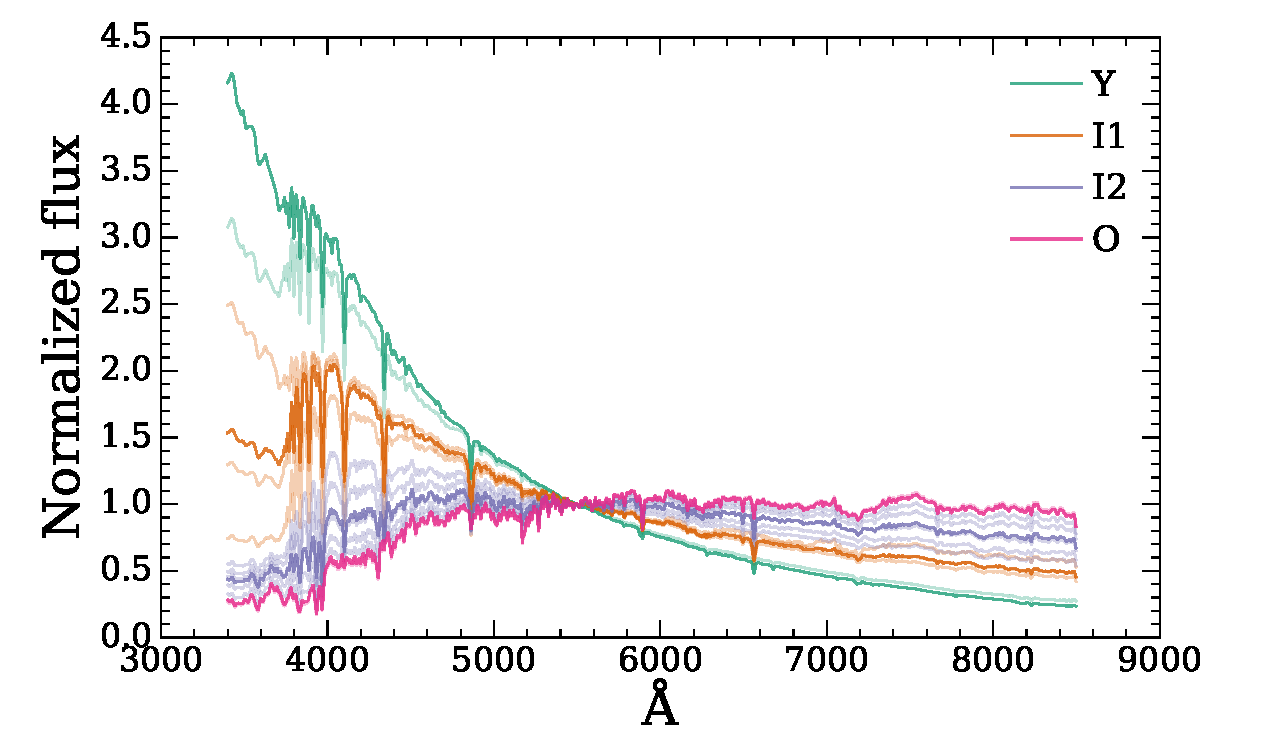
\includegraphics[width=\columnwidth]{891_2/figs/bc_dfk_comp.pdf}
  \caption[Comparison of full BC03 and diffusion k-means
    spectra]{\fixspacing\label{891_2:fig:bc_dfk_comp}The set of
    \citetalias{Bruzual03} SSPs used in \S\ref{891_2:sec:bc03_SSP}
    (lightly shaded) and the reduced basis set that results from
    applying diffusion k-means (solid). The colors correspond to the
    final groupings in diffusion K-means space (defined in Table
    \ref{891_2:tab:dfk}). Figure adapted from \citetalias{Mosby15}.}
\end{figure}

Despite being based on purely statistical methods (i.e., diffusion
k-means), the age groupings of the final bins roughly correspond to
important timescales in stellar evolution. The Young bin corresponds
to the very brightest O and B stars that have strong UV flux and
prominant Balmer absorption. Intermediate 1 covers B, A, and F stars
that have the strongest Balmer absorption. Intermediate 2 covers
timescales where the main sequence turn-off transitions from A stars
to late F stars and the total flux has major contributions from giant
branch and thermally pulsating asymptotic giant branch stars. Finally,
the Old bin contains F and G stars with strong metal lines and very
little spectral evolution over the bin. It is important to note that
\citetalias{Mosby15} do artificially adjust the limits of the oldest
two bins to account for the fact that star formation histories are
rarely constant over \val{10}{Gyr}.

%+++++++++++++++=
%% {\bf MAB: Check your MS evolutionary time-scales. I think Y includes
%%   O/B, while I1 includes B/A/F. For the I2 bin a lot happens. This is
%%   the time scale over which TP-AGB stars have significant
%%   contriutions, the bolometric flux becomes dominated by the giant
%%   branch (beyhond 1-2 Gyr), and the MS turn-off evolves from A into
%%   late F. In the oldest bin, everthing is boring; the turn-off has
%%   ground down to somewhere between late F and early G, while the red
%%   light is dominated by red giants. Might think about where HB becomes
%%   important which will be even more sensitive to metallicity than the
%%   RGB. Blue HB can compete with MS turn-off in the blue/NUV.

%%   I don't understand the statement in the last sentence for why the
%%   limits in the two oldest bins were adjusted. I actually think this
%%   is likely a mistake since 0.4-2 Gyr is likely the key phase in which
%%   TP-AGB stars play a role.

%%   On this point I asked about the wave range for establishing DFK
%%   because if it did not go very red and used BC03 it may not have been
%%   sensitive to TP-AGB. So among the limitations of the DFK that can be
%%   improved upon in the future is the treatment of metallicity
%%   variations, extention to longer wavelengths, and application to
%%   other SPS models (especially MA11) that are sensitive to variations
%%   in intermediate age populations.

%% }

One of the current limitations of this method is that the diffusion k-means
grouping has so far only been performed on solar metallicity SSPs. To
constrain metallicity we construct composite metallicity libraries in the
style of both \S\ref{891_2:sec:mono_metal} and \S\ref{891_2:sec:multi_metal} using the
exact same SSP groupings described in Table \ref{891_2:tab:dfk}. The resulting
analysis is the same as for those sections. In this sense the DFK grouping
only reduces the size of the age dimension of SSP parameter space; we still
need to deal with uncertainties in the choice of metallicity and degeneracies
between age and metallicity.

\subsection{Alternative SSP templates}
\label{891_2:sec:ma11}

The SSPs of \citet{Maraston11} (hereafter \citetalias{Maraston11})
offer an appealing, modern alternative to the \citetalias{Bruzual03}
SSPs. Namely, they avoid the known issues with Balmer apsorption in
the Stelib library \citep{Groves11} by using the MILES stellar
libraries \citep{Vazdekis10,Falcon-Barroso11}. \citetalias{Maraston11}
also use the fuel consumption theorem
\citep{Renzini81,Buzzoni89,Maraston05} to address problems that arise
from using isochrones (as do \citetalias{Bruzual03}) to simulate the
rapid changes in phase that occur at the tip of the RGB, the AGB, and
thr RGB bump.

To make as fair a comparison as possible the \citetalias{Maraston11}
models were first grouped into the same diffusion k-means bins as the
BC03 models (the consequences of using a DFK grouping from a different
set of models will be ignored for the time being). This decision comes
with one major caveat; the \citetalias{Maraston11} models do not
extend to the youngest ages sampled by \citetalias{Bruzual03}. The
youngest \citetalias{Maraston11} age is \val{6.5}{Myr}, which is
\emph{older} than the youngest bin found by \citetalias{Mosby15}. For
this reason our \citetalias{Maraston11} basis set does not have a
``Young'' SSP and thus consists of only 3 SSPs for each metallicity.

\begin{figure}
  \centering
  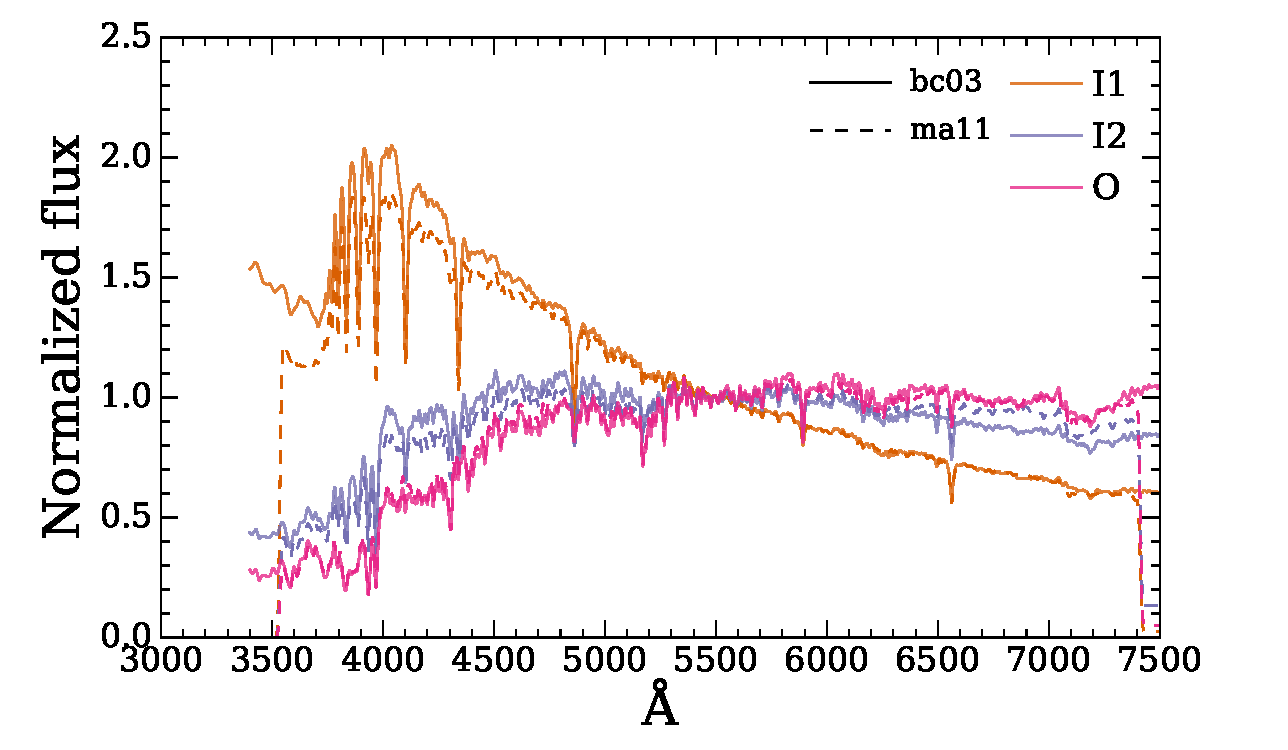
\includegraphics[width=\columnwidth]{891_2/figs/ma_bc_comp.pdf}
  \caption[Comparison of DFK BC03 and MA11 SSP template
    libraries]{\fixspacing\label{891_2:fig:ma_bc_comp}Comparison of
    diffusion k-means \citetalias{Bruzual03} and
    \citetalias{Maraston11} models. Colors correspond to DFK age bins,
    as defined in Table \ref{891_2:tab:dfk}. The solid and dashed
    lines are the \citetalias{Bruzual03} and \citetalias{Maraston11}
    basis sets, respectively. Note that the \citetalias{Maraston11}
    basis set lacks the youngest age bin.{\bf MAB: Very hard to see
      differences between spectra. Maybe only plot I1, I2, and O and
      zoom in y. Also limit wavelength range to what can be computed
      for Ma11.}}
\end{figure}

Figure \ref{891_2:fig:ma_bc_comp} shows a comparison between the
\citetalias{Maraston11} and \citetalias{Bruzual03} SSP basis sets at
\val{1}{\Zsol}. The differences in the shapes of these two basis sets
have important implications for the interpretation of the SSP fitting
results. In particular, the difference between the two models in the
blue end decreases with SSP age; the I2 \citetalias{Maraston11} SSP
has less flux than the I2 \citetalias{Bruzual03} SSP by a larger
difference than the I1 SSPs. At the oldest SSP age the
\citetalias{Maraston11} model actually produces slightly more flux
than the \citetalias{Bruzual03} model. Because of this trend the
\citetalias{Maraston11} require more mass at younger ages to match the
same spectrum as the \citetalias{Bruzual03} basis. Thus we expect the
derived $\tau_L$ values for the \citetalias{Maraston11} basis set to
be lower than those derived using \citetalias{Bruzual03} SSPs.

%+++++++++++
%% {\bf MAB: How much of the above should we say is highly dependent on
%%   the fact that we have not really done a full-up DFK on the
%%   \citetalias{Maraston11} models but are imposing the age-bins defined
%%   by M15's analysis of BC03? I.e., the differences we are finding here
%%   may not be as important or significant.}

In addition to the lack of young ages the age resolution of
\citetalias{Maraston11} is much less than
\citetalias{Bruzual03}. Compared to \citetalias{Bruzual03}'s 107 age
bins the \citetalias{Maraston11} have at most 50 age bins (for solar
metallicity) and sometimes as few as 14. To asses whether this limited
age sampling affects the diffusion k-means averages we rebinned the
\citetalias{Bruzual03} diffusion k-means spectra from a sample of
\citetalias{Bruzual03} spectra down-selected to match the age bins of
the \citetalias{Maraston11} models. Figure \ref{891_2:fig:bc03_downselect}
shows a comparison of the \citetalias{Maraston11} and
\citetalias{Bruzual03} DFK models; down-selecting the
\citetalias{Bruzual03} models does not appreciably affect the final,
averaged DFK spectra.

Ultimately, we choose not to use the DFK'd \citetalias{Maraston11}
models, but this is primarily due to the fact that our DFK bins are
constructed specifically for the \citetalias{Bruzual03} data set. The
omission of \citetalias{Maraston11} models from subsequent analysis is
not a statement about the quality of the models themselves. We
strongly warn the reader away from making a robust comparison between
the models of \citetalias{Bruzual03} and \citetalias{Maraston11} based
on our analysis precisely for the reason that our DFK binning was
tailored for the \citetalias{Bruzual03} models.  Future work in the
area of diffusion k-means should be able to easily produce a separate
set of DFK basis spectra for the full \citetalias{Maraston11} model
set.

%++++++++++++++++++
%% {\bf MAB: I would rewrite the ``omission'' sentence. I think there are
%%   three concerns we have had with the Maraston models (1) the
%%   time-steps were coarser; (2) the time steps didn't go as young ages;
%%   (3) th DFK analysis was not done with these models. We've eliminated
%%   (1) as an issues, but as we will find in Fig 21, the youngest DFK
%%   does seem important at low heights. Given that the DFK analysis was
%%   done with the BC03 data and has this younger age bin it is prudent
%%   to continue with the BC03 spectra. However, future analysis needs to
%%   consider the \citetalias{Maraston11} models, particularly for
%%   intermediate ages when extending farther to the read where TP-AGB
%%   stars are more important.}

\begin{figure}
  \centering
  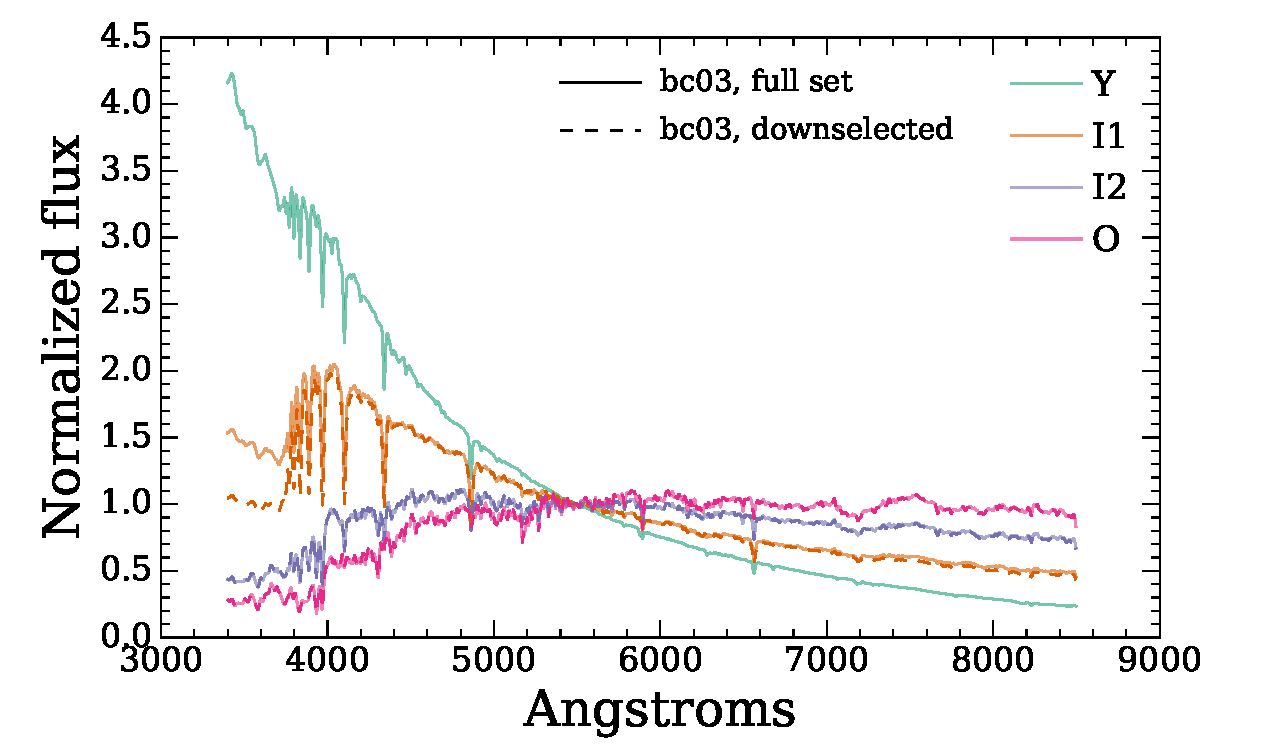
\includegraphics[width=\columnwidth]{891_2/figs/bc_downselect.pdf}
  \caption[Effect of downselecting BC03 age
    resolution]{\fixspacing\label{891_2:fig:bc03_downselect}The effect
    of downselecting the \citetalias{Bruzual03} ages to match the age
    grid of the \citetalias{Maraston11} models. This down-selection
    reduced the number of input SSPs from 107 to 50. Note that the
    \citetalias{Maraston11} age grid does not contain the youngest age
    bin.}
\end{figure}

\subsection{The final choice of SSP basis set}
\label{891_2:sec:final_SSP}
\begin{figure}
  \centering
  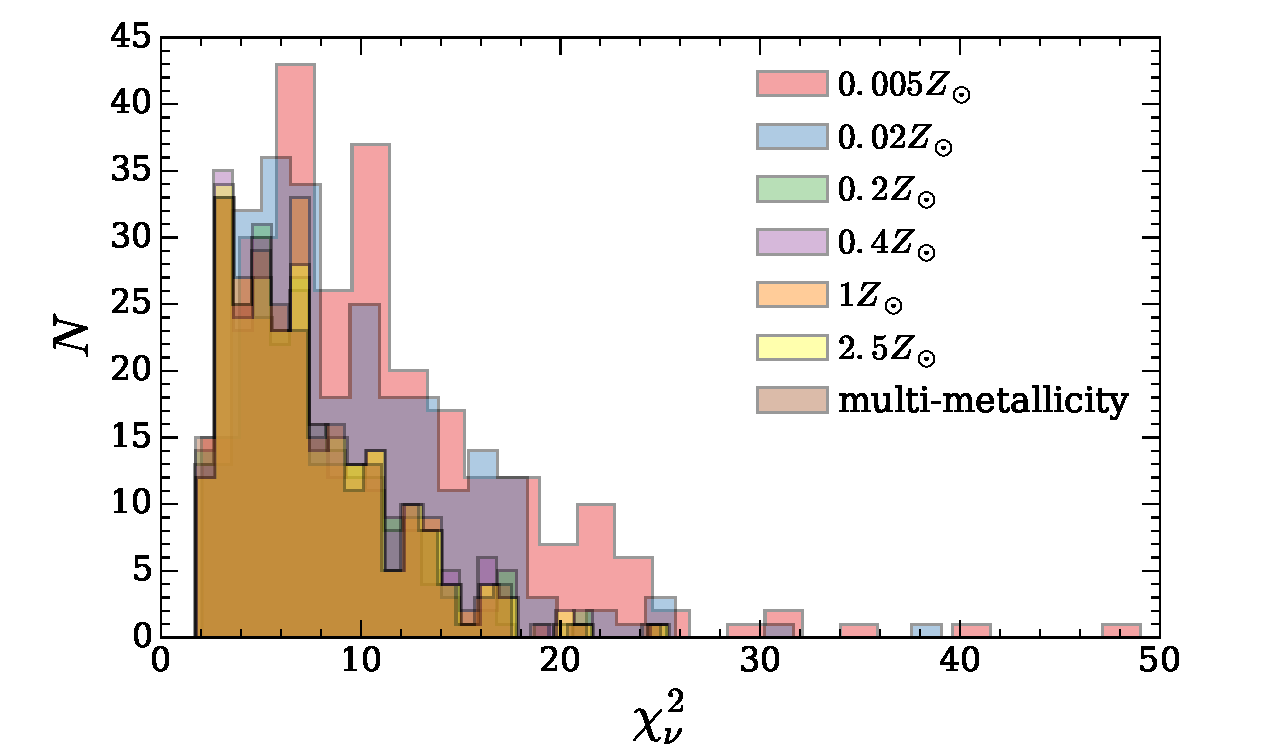
\includegraphics[width=\columnwidth]{891_2/figs/dfk_chihist.pdf}
  \caption[$\chi_{\nu}^2$ distributions for different metallcity
    fits]{\fixspacing\label{891_2:fig:chisq_hist}Histograms of
    best-fitting $\chi^2_\nu$ values for all 261 apertures using both
    mono-metallicity and multi-metallicity DFK SSP library sets.}
\end{figure}

We choose the \citetalias{Bruzual03} DFK model set as our primary SSP
library because it is statisticalyl motivated, reduces the number of
fit free parameters (which also reduced computation time), and
approximates important epochs in stellar evolution. We do note,
however, that the DFK bins presented in \citetalias{Mosby15} are
designed for very low signal to noise data and therefore may reduce
the number of SSP templates beyond what is strictly necessary for our
data. In particular the I2 DFK bin covers a very wide range in stellar
evolution and future work might show that it can be split into
multiple bins.

%++++++++++++++
%% {\bf MAB: with a nod to the lack of an intermediate age bin, i.e.,
%%   room for future improvement. I think this or somewhere we need to
%%   recount that M15 analysis was based on VERY low S/N, so we have to
%%   explain why we think this coarse age grid is reaonably using
%%   available information with our data. (This is a major point,
%%   actually.)}

We modify the solar metallicity basis set defined by
\citetalias{Mosby15} to consider multiple metallicities using the same
method decribed in \S\ref{891_2:sec:multi_metal}; each age bin is allowed to
contribute light from an arbitrary number of SSPs with different
metallicities. Thus the full set contains 24 separate SSPs: six
metallicities each in the four age bins described by
\citetalias{Mosby15}. We find, however, that SSPs with metallicity
below \val{0.2}{\Zsol} are both statistically unrepresentative of our
galaxy spectra and astrophysically astrophysically implausible given
expected rapid chemical enrichment time-scales and therefore the
minimal contribution from super metal-poor populations to the
integrated light.

To test this assertion we construct mono-metallicity DFK basis sets in
the same metallicity bins listed in \S\ref{891_2:sec:mono_metal} and fit
them to our data. We then compare the distributions of goodness-of-fit
(i.e., $\chi^2_\nu$) between the different metallicities and can
identify fits that are statistically different from the best fitting
model and therefore not likely representative of the true galaxy
spectrum.

Figure \ref{891_2:fig:chisq_hist} shows the $\chi^2_\nu$ distributions for
all \GP apertures for the mono-metallicity DFK basis sets and our
final choice of SSP basis set (``multi-metallicity''). The two lowest
mono-metallicity SSP sets (0.005 and \val{0.02}{\Zsol}) produce
spectral fits that occupy a different locus in $\chi^2_\nu$ and are
worse than all other metallicities. A 2-sample KS test confrims that
these two metallcities are not part of the same distribution as the
other mono-metallicity basis sets with $p \ll 0.001$. Conversely, all
other mono-metallicity basis sets are drawn from the same underlying
distribution with $p > 0.8$, in the worst case, and it is therefore
difficult to justify, in a statistical sense, choosing a single
metallicity over another. 

Figure \ref{891_2:fig:chisq_hist} also shows that our final,
multi-metallicity basis set (with only $Z \geq \val{0.2}{\Zsol}$)
produces fits of comparable quality to the mono-metallicity fits ($p >
0.8$). Thus we cannot say that our multi-metallicity basis set provide
a statistical improvement over any one mono-metallicity basis set. The
advantage, however, of the final basis set is in the physical insight
gained by creating a more realistic physical model of the
galaxy. Using a multi-metallicity SSP set also allows us to check if
astrophysically reasonable age-metallicity relations come out of our
analysis \emph{without} having to assume age/metallicity priors (as is
done in mono-metallicity basis sets). In other words, both mono and
multi-metallcity basis sets will be subject to degeneracies between
age and metallicity, but we can only quantify these degeneracies
(\S\ref{891_2:sec:fit_err}) with a multi-metallicity basis set.

%+++++++++++++++++++
%% {\bf MAB: Let me make sure I understand the histogram and
%%   comparison. For each mono-z case you are plotting the $\chi^2_\nu$
%%   distribution for fits with that metallicity to every aperture
%%   (individually). That means the $\chi^2_\nu$ distribution is
%%   statistically the same as the multi-Z case, where the mean Z is
%%   tailored for each galaxy. At first blush, that ain't good. It would
%%   suggest we have jack for leverage on Z. One related aside: How does
%%   the multi-z histogram compare to one where for every aperture you
%%   take the lowest mono-z $\chi^2_\nu$ value across all Z?

%%   Here is what I think we need to say. First, the reason why we think
%%   the $\chi^2_\nu$ distributions are so similar is because of the
%%   well-known age-Z degeneracy. Hence our exploration here is to
%%   eliminate as much Z and age that we think is either implausible
%%   (low-Z) or for which we have inadequate information to resolve (DFK
%%   age bins). With that in hand we want to use the multi-Z models to
%%   determine if astrophysically plausible age-metallicity relations
%%   come out of the analysis w/o further priors; we couldn't explore
%%   this with the mono-z models. Second, one of the reasons why we
%%   looked at altering $\chi^2$ was specifically to determine if we could
%%   improve the age-Z discrimination. This motivates the next section.

%---------------------
%%   Also, I think we talked about two side-by-side historgrams: One
%%   showing all mono-Z for $Z>0.02$ and multi-Z averaged together vs the
%%   two low-Z cases; and then on blowing up in $\chi^2_\nu$ comparing
%%   the mono-z with multi-z. I still think that is a good idea.

%% }

Finally, Figure \ref{891_2:fig:ex_fit} shows an example of the best
fit in one aperture (pointing 6, aperture 9). This example is typical
for most apertures in our data set; the data has relatively high
signal/noise and is well fit by the superposition of our final SSP
basis set.

%-----------------
%% {\bf MAB: For the figure we discussed the idea of putting in a few
%%   apertures with different characteristic ages. Also, coul you label
%%   the lines by DFK age and Z as well as the L-weighted total values?
%%   You should also show a residual spectrum at the bottom of each panel
%%   (for each aperture.}

\begin{figure}
  \centering
  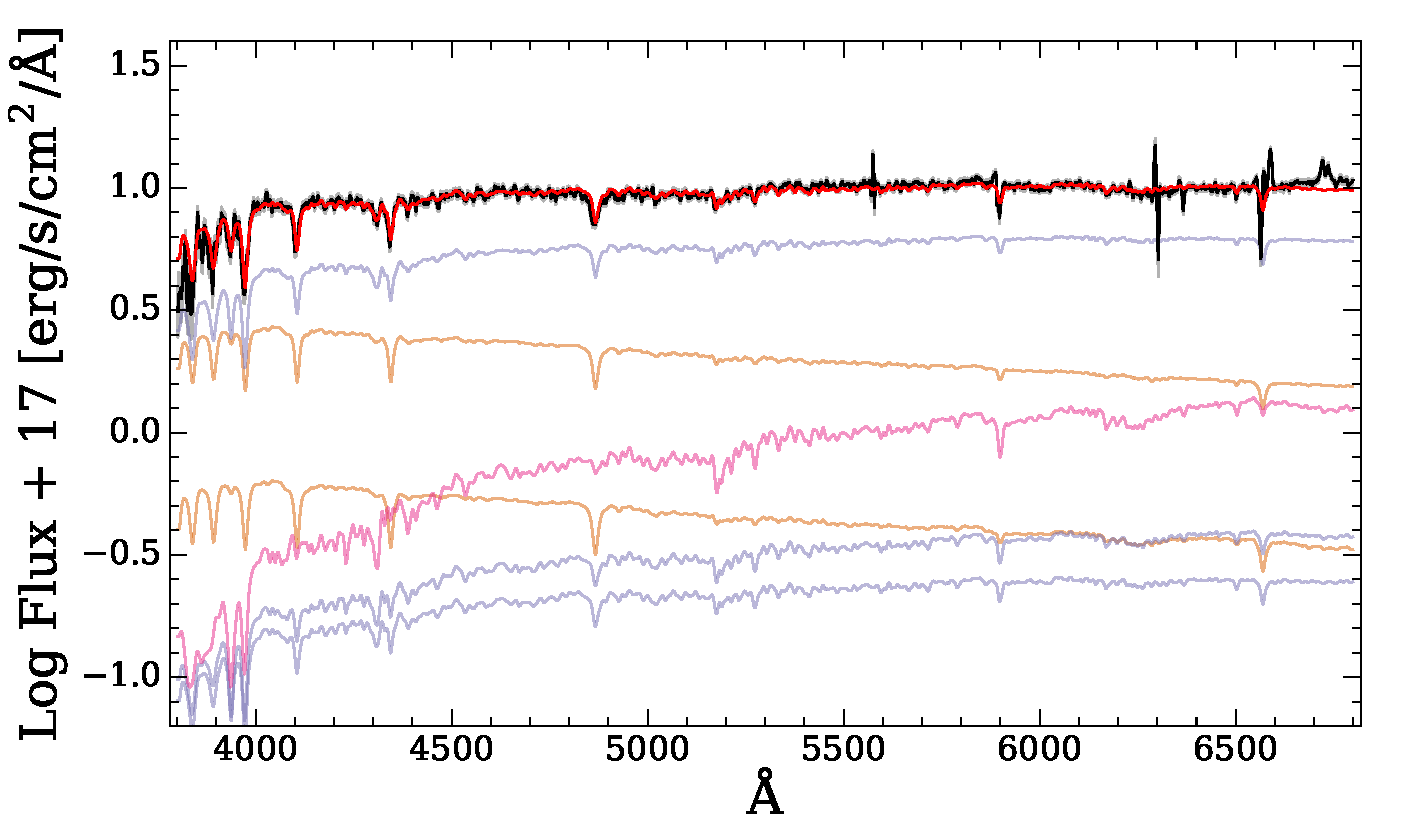
\includegraphics[width=\columnwidth]{891_2/figs/example_fit.pdf}
  \caption[Example model galaxy
    fit]{\fixspacing\label{891_2:fig:ex_fit}Example SSP fit to a
    single galaxy aperture (P6.9). The black line with gray shading
    (hard to see) show the measured flux and corresponding
    uncertainty. Each colored line (besides red) is an SSP from the
    \citetalias{Bruzual03} DFK basis set described above and the
    colors are the same as in Figure \ref{891_2:fig:bc_dfk_comp}. The
    red line is the superposition of all the individual SSP spectra.}
\end{figure}
